6. Расставьте скобки так, чтобы равенство было верным: $20:2+7\cdot2-5=29.$
\newpage
\noindent7. Разместите числа 1, 2, 3, 4, 5, 6, 7, 8, 9 в пустых кружках так, чтобы сумма трёх чисел расположенных на каждой прямой, была равна 15.
\begin{center}
\begin{figure}[h!]
\center{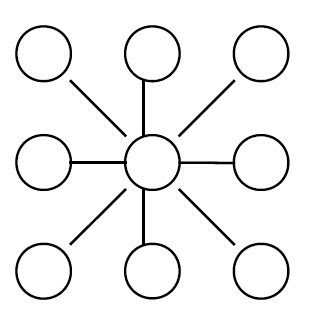
\includegraphics[scale=0.35]{2.png}}
\end{figure}
\end{center}
